\documentclass[twoside]{book}

% Packages required by doxygen
\usepackage{fixltx2e}
\usepackage{calc}
\usepackage{doxygen}
\usepackage[export]{adjustbox} % also loads graphicx
\usepackage{graphicx}
\usepackage[utf8]{inputenc}
\usepackage{makeidx}
\usepackage{multicol}
\usepackage{multirow}
\PassOptionsToPackage{warn}{textcomp}
\usepackage{textcomp}
\usepackage[nointegrals]{wasysym}
\usepackage[table]{xcolor}

% Font selection
\usepackage[T1]{fontenc}
\usepackage[scaled=.90]{helvet}
\usepackage{courier}
\usepackage{amssymb}
\usepackage{sectsty}
\renewcommand{\familydefault}{\sfdefault}
\allsectionsfont{%
  \fontseries{bc}\selectfont%
  \color{darkgray}%
}
\renewcommand{\DoxyLabelFont}{%
  \fontseries{bc}\selectfont%
  \color{darkgray}%
}
\newcommand{\+}{\discretionary{\mbox{\scriptsize$\hookleftarrow$}}{}{}}

% Page & text layout
\usepackage{geometry}
\geometry{%
  a4paper,%
  top=2.5cm,%
  bottom=2.5cm,%
  left=2.5cm,%
  right=2.5cm%
}
\tolerance=750
\hfuzz=15pt
\hbadness=750
\setlength{\emergencystretch}{15pt}
\setlength{\parindent}{0cm}
\setlength{\parskip}{3ex plus 2ex minus 2ex}
\makeatletter
\renewcommand{\paragraph}{%
  \@startsection{paragraph}{4}{0ex}{-1.0ex}{1.0ex}{%
    \normalfont\normalsize\bfseries\SS@parafont%
  }%
}
\renewcommand{\subparagraph}{%
  \@startsection{subparagraph}{5}{0ex}{-1.0ex}{1.0ex}{%
    \normalfont\normalsize\bfseries\SS@subparafont%
  }%
}
\makeatother

% Headers & footers
\usepackage{fancyhdr}
\pagestyle{fancyplain}
\fancyhead[LE]{\fancyplain{}{\bfseries\thepage}}
\fancyhead[CE]{\fancyplain{}{}}
\fancyhead[RE]{\fancyplain{}{\bfseries\leftmark}}
\fancyhead[LO]{\fancyplain{}{\bfseries\rightmark}}
\fancyhead[CO]{\fancyplain{}{}}
\fancyhead[RO]{\fancyplain{}{\bfseries\thepage}}
\fancyfoot[LE]{\fancyplain{}{}}
\fancyfoot[CE]{\fancyplain{}{}}
\fancyfoot[RE]{\fancyplain{}{\bfseries\scriptsize Generated by Doxygen }}
\fancyfoot[LO]{\fancyplain{}{\bfseries\scriptsize Generated by Doxygen }}
\fancyfoot[CO]{\fancyplain{}{}}
\fancyfoot[RO]{\fancyplain{}{}}
\renewcommand{\footrulewidth}{0.4pt}
\renewcommand{\chaptermark}[1]{%
  \markboth{#1}{}%
}
\renewcommand{\sectionmark}[1]{%
  \markright{\thesection\ #1}%
}

% Indices & bibliography
\usepackage{natbib}
\usepackage[titles]{tocloft}
\setcounter{tocdepth}{3}
\setcounter{secnumdepth}{5}
\makeindex

% Hyperlinks (required, but should be loaded last)
\usepackage{ifpdf}
\ifpdf
  \usepackage[pdftex,pagebackref=true]{hyperref}
\else
  \usepackage[ps2pdf,pagebackref=true]{hyperref}
\fi
\hypersetup{%
  colorlinks=true,%
  linkcolor=blue,%
  citecolor=blue,%
  unicode%
}

% Custom commands
\newcommand{\clearemptydoublepage}{%
  \newpage{\pagestyle{empty}\cleardoublepage}%
}

\usepackage{caption}
\captionsetup{labelsep=space,justification=centering,font={bf},singlelinecheck=off,skip=4pt,position=top}

%===== C O N T E N T S =====

\begin{document}

% Titlepage & ToC
\hypersetup{pageanchor=false,
             bookmarksnumbered=true,
             pdfencoding=unicode
            }
\pagenumbering{alph}
\begin{titlepage}
\vspace*{7cm}
\begin{center}%
{\Large My Project }\\
\vspace*{1cm}
{\large Generated by Doxygen 1.8.13}\\
\end{center}
\end{titlepage}
\clearemptydoublepage
\pagenumbering{roman}
\tableofcontents
\clearemptydoublepage
\pagenumbering{arabic}
\hypersetup{pageanchor=true}

%--- Begin generated contents ---
\chapter{Hierarchical Index}
\section{Class Hierarchy}
This inheritance list is sorted roughly, but not completely, alphabetically\+:\begin{DoxyCompactList}
\item \contentsline{section}{Icp\+Map\+Maker}{\pageref{classIcpMapMaker}}{}
\item \contentsline{section}{Localisation\+Method}{\pageref{classLocalisationMethod}}{}
\begin{DoxyCompactList}
\item \contentsline{section}{Graph\+Optimiser}{\pageref{classGraphOptimiser}}{}
\end{DoxyCompactList}
\item \contentsline{section}{Localiser}{\pageref{classLocaliser}}{}
\item \contentsline{section}{Observer}{\pageref{classObserver}}{}
\begin{DoxyCompactList}
\item \contentsline{section}{G\+N\+S\+S\+Observation}{\pageref{classGNSSObservation}}{}
\item \contentsline{section}{I\+C\+P\+Observation}{\pageref{classICPObservation}}{}
\end{DoxyCompactList}
\item \contentsline{section}{Predictor}{\pageref{classPredictor}}{}
\begin{DoxyCompactList}
\item \contentsline{section}{Imu\+Measurement}{\pageref{classImuMeasurement}}{}
\item \contentsline{section}{Speed\+Measurement}{\pageref{classSpeedMeasurement}}{}
\end{DoxyCompactList}
\item \contentsline{section}{R\+O\+S\+Localiser}{\pageref{classROSLocaliser}}{}
\item \contentsline{section}{Simple\+\_\+graph}{\pageref{classSimple__graph}}{}
\item \contentsline{section}{Simple\+\_\+node}{\pageref{structSimple__node}}{}
\end{DoxyCompactList}

\chapter{Class Index}
\section{Class List}
Here are the classes, structs, unions and interfaces with brief descriptions\+:\begin{DoxyCompactList}
\item\contentsline{section}{\hyperlink{classGNSSObservation}{G\+N\+S\+S\+Observation} }{\pageref{classGNSSObservation}}{}
\item\contentsline{section}{\hyperlink{classGraphOptimiser}{Graph\+Optimiser} \\*Optimise a graph of poses Optimises a graph structure containing poses linked by relative motion, with additional edges for global observations }{\pageref{classGraphOptimiser}}{}
\item\contentsline{section}{\hyperlink{classIcpMapMaker}{Icp\+Map\+Maker} }{\pageref{classIcpMapMaker}}{}
\item\contentsline{section}{\hyperlink{classICPObservation}{I\+C\+P\+Observation} }{\pageref{classICPObservation}}{}
\item\contentsline{section}{\hyperlink{classImuMeasurement}{Imu\+Measurement} }{\pageref{classImuMeasurement}}{}
\item\contentsline{section}{\hyperlink{classLocalisationMethod}{Localisation\+Method} }{\pageref{classLocalisationMethod}}{}
\item\contentsline{section}{\hyperlink{classLocaliser}{Localiser} \\*The class that manages the localisation process }{\pageref{classLocaliser}}{}
\item\contentsline{section}{\hyperlink{classObserver}{Observer} \\*The base class for providing observations Class type that gives an observation of the current robot pose in the global frame of reference }{\pageref{classObserver}}{}
\item\contentsline{section}{\hyperlink{classPredictor}{Predictor} \\*The base class for predictive inputs Class type that gives an informed prediction about the future relative location of the robot (given some relative sensor information) }{\pageref{classPredictor}}{}
\item\contentsline{section}{\hyperlink{classROSLocaliser}{R\+O\+S\+Localiser} \\*The class that manages the localisation process }{\pageref{classROSLocaliser}}{}
\item\contentsline{section}{\hyperlink{classSimple__graph}{Simple\+\_\+graph} }{\pageref{classSimple__graph}}{}
\item\contentsline{section}{\hyperlink{structSimple__node}{Simple\+\_\+node} }{\pageref{structSimple__node}}{}
\item\contentsline{section}{\hyperlink{classSpeedMeasurement}{Speed\+Measurement} }{\pageref{classSpeedMeasurement}}{}
\end{DoxyCompactList}

\chapter{Class Documentation}
\hypertarget{classGNSSObservation}{}\section{G\+N\+S\+S\+Observation Class Reference}
\label{classGNSSObservation}\index{G\+N\+S\+S\+Observation@{G\+N\+S\+S\+Observation}}


Inheritance diagram for G\+N\+S\+S\+Observation\+:
\nopagebreak
\begin{figure}[H]
\begin{center}
\leavevmode
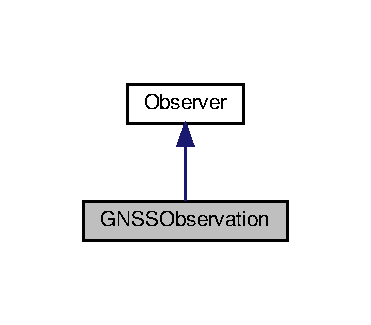
\includegraphics[width=178pt]{classGNSSObservation__inherit__graph}
\end{center}
\end{figure}


Collaboration diagram for G\+N\+S\+S\+Observation\+:
\nopagebreak
\begin{figure}[H]
\begin{center}
\leavevmode
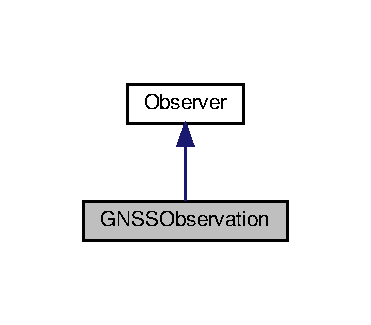
\includegraphics[width=178pt]{classGNSSObservation__coll__graph}
\end{center}
\end{figure}
\subsection*{Public Member Functions}
\begin{DoxyCompactItemize}
\item 
\mbox{\Hypertarget{classGNSSObservation_afd04d0b5d0a942a4402e00bb1748e1df}\label{classGNSSObservation_afd04d0b5d0a942a4402e00bb1748e1df}} 
void {\bfseries receive\+\_\+message} (const sensor\+\_\+msgs\+::\+Nav\+Sat\+Fix\+::\+Const\+Ptr \&msg)
\end{DoxyCompactItemize}
\subsection*{Public Attributes}
\begin{DoxyCompactItemize}
\item 
\mbox{\Hypertarget{classGNSSObservation_a40403a43f71cb41d34964ad7b5312e83}\label{classGNSSObservation_a40403a43f71cb41d34964ad7b5312e83}} 
const double {\bfseries R\+T\+K\+\_\+\+C\+O\+V\+A\+R\+I\+A\+N\+C\+E\+\_\+\+T\+H\+R\+E\+S\+H\+O\+LD} = 0.\+001
\item 
\mbox{\Hypertarget{classGNSSObservation_a565aa2d16a03d46821af8dfb270e6b09}\label{classGNSSObservation_a565aa2d16a03d46821af8dfb270e6b09}} 
const double {\bfseries P\+O\+S\+I\+T\+I\+O\+N\+\_\+\+C\+O\+V\+A\+R\+I\+A\+N\+C\+E\+\_\+\+G\+N\+SS} = pow(2.\+5, 2)
\item 
\mbox{\Hypertarget{classGNSSObservation_a2e7aa6fd27ee685def43309596899da9}\label{classGNSSObservation_a2e7aa6fd27ee685def43309596899da9}} 
const double {\bfseries P\+O\+S\+I\+T\+I\+O\+N\+\_\+\+C\+O\+V\+A\+R\+I\+A\+N\+C\+E\+\_\+\+R\+TK} = pow(0.\+5, 2)
\item 
\mbox{\Hypertarget{classGNSSObservation_af2032110626cec0239c5920e65e68ccc}\label{classGNSSObservation_af2032110626cec0239c5920e65e68ccc}} 
const double {\bfseries H\+E\+A\+D\+I\+N\+G\+\_\+\+C\+O\+V\+A\+R\+I\+A\+N\+CE} = pow(2. $\ast$ (3.\+1417/180.), 2)
\end{DoxyCompactItemize}


The documentation for this class was generated from the following file\+:\begin{DoxyCompactItemize}
\item 
/home/stew/src/catkin/src/localiser/include/localiser/observer.\+hpp\end{DoxyCompactItemize}

\hypertarget{classGraphOptimiser}{}\section{Graph\+Optimiser Class Reference}
\label{classGraphOptimiser}\index{Graph\+Optimiser@{Graph\+Optimiser}}


Optimise a graph of poses Optimises a graph structure containing poses linked by relative motion, with additional edges for global observations.  




{\ttfamily \#include $<$graph\+\_\+optimiser.\+hpp$>$}



Inheritance diagram for Graph\+Optimiser\+:
\nopagebreak
\begin{figure}[H]
\begin{center}
\leavevmode
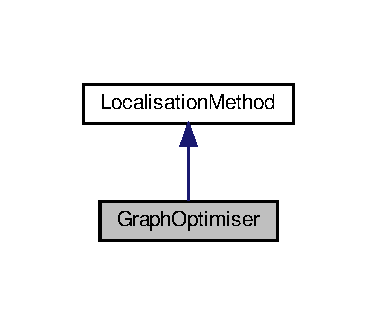
\includegraphics[width=181pt]{classGraphOptimiser__inherit__graph}
\end{center}
\end{figure}


Collaboration diagram for Graph\+Optimiser\+:
\nopagebreak
\begin{figure}[H]
\begin{center}
\leavevmode
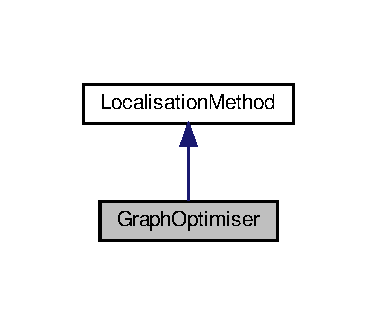
\includegraphics[width=181pt]{classGraphOptimiser__coll__graph}
\end{center}
\end{figure}
\subsection*{Public Member Functions}
\begin{DoxyCompactItemize}
\item 
\mbox{\Hypertarget{classGraphOptimiser_a986c07622d992bcf4ea4b6711a025b5e}\label{classGraphOptimiser_a986c07622d992bcf4ea4b6711a025b5e}} 
void {\bfseries Run\+Optimiser} ()
\item 
Eigen\+::\+Vector3d \hyperlink{classGraphOptimiser_a3310a9869b3cec56fb9ccc6a0c944e15}{Vehicle\+Model} (Eigen\+::\+Vector3d \&current\+\_\+pose, Eigen\+::\+Vector2d \&motion\+\_\+delta)
\item 
void \hyperlink{classGraphOptimiser_ad856bbb20088fae667b00f8ef0355f32}{Add\+Relative\+Motion} (Eigen\+::\+Vector2d \&motion, Eigen\+::\+Vector2d \&covariance, ros\+::\+Time stamp)
\begin{DoxyCompactList}\small\item\em Perform the optimisation. \end{DoxyCompactList}\item 
void \hyperlink{classGraphOptimiser_addfbfde9e277dd61876e64fd23c7eae8}{Add\+Absolute\+Position} (Eigen\+::\+Vector3d \&observation, Eigen\+::\+Vector3d \&covariance, ros\+::\+Time stamp)
\end{DoxyCompactItemize}
\subsection*{Public Attributes}
\begin{DoxyCompactItemize}
\item 
\mbox{\Hypertarget{classGraphOptimiser_ad1b6ee44cbaa3b3d2817d62acbdfd7d6}\label{classGraphOptimiser_ad1b6ee44cbaa3b3d2817d62acbdfd7d6}} 
Eigen\+::\+Matrix3d {\bfseries gps\+\_\+information}
\item 
\mbox{\Hypertarget{classGraphOptimiser_a1fae664a0b8570d2f88392662dde3710}\label{classGraphOptimiser_a1fae664a0b8570d2f88392662dde3710}} 
mrpt\+::obs\+::\+C\+Action\+Robot\+Movement2\+D\+::\+T\+Motion\+Model\+Options {\bfseries motion\+\_\+model\+\_\+options\+\_\+}
\item 
\mbox{\Hypertarget{classGraphOptimiser_a6247045a0b2757e02690a8e98ef71b03}\label{classGraphOptimiser_a6247045a0b2757e02690a8e98ef71b03}} 
g2o\+::\+Vertex\+S\+E2 $\ast$ {\bfseries origin}
\item 
\mbox{\Hypertarget{classGraphOptimiser_ab1f61ad8e5e6c8bada0263942b1b068c}\label{classGraphOptimiser_ab1f61ad8e5e6c8bada0263942b1b068c}} 
uint32\+\_\+t {\bfseries current\+\_\+index}
\item 
\mbox{\Hypertarget{classGraphOptimiser_a240a79573703fa7c1c6ab1ddb7dfc601}\label{classGraphOptimiser_a240a79573703fa7c1c6ab1ddb7dfc601}} 
double {\bfseries datum\+\_\+x}
\item 
\mbox{\Hypertarget{classGraphOptimiser_a36a019181bf4711ba275398413eff289}\label{classGraphOptimiser_a36a019181bf4711ba275398413eff289}} 
double {\bfseries datum\+\_\+y}
\item 
\mbox{\Hypertarget{classGraphOptimiser_a6eb72ad8bf9d692c2b0daf64f45c8cce}\label{classGraphOptimiser_a6eb72ad8bf9d692c2b0daf64f45c8cce}} 
uint32\+\_\+t {\bfseries previous\+\_\+odom\+\_\+vertex\+\_\+id}
\item 
\mbox{\Hypertarget{classGraphOptimiser_ad4772e6892e2c1cfca68bfbdce804c6e}\label{classGraphOptimiser_ad4772e6892e2c1cfca68bfbdce804c6e}} 
g2o\+::\+Sparse\+Optimizer {\bfseries global\+\_\+optimizer}
\end{DoxyCompactItemize}


\subsection{Detailed Description}
Optimise a graph of poses Optimises a graph structure containing poses linked by relative motion, with additional edges for global observations. 

\subsection{Member Function Documentation}
\mbox{\Hypertarget{classGraphOptimiser_addfbfde9e277dd61876e64fd23c7eae8}\label{classGraphOptimiser_addfbfde9e277dd61876e64fd23c7eae8}} 
\index{Graph\+Optimiser@{Graph\+Optimiser}!Add\+Absolute\+Position@{Add\+Absolute\+Position}}
\index{Add\+Absolute\+Position@{Add\+Absolute\+Position}!Graph\+Optimiser@{Graph\+Optimiser}}
\subsubsection{\texorpdfstring{Add\+Absolute\+Position()}{AddAbsolutePosition()}}
{\footnotesize\ttfamily void Graph\+Optimiser\+::\+Add\+Absolute\+Position (\begin{DoxyParamCaption}\item[{Eigen\+::\+Vector3d \&}]{observation,  }\item[{Eigen\+::\+Vector3d \&}]{covariance,  }\item[{ros\+::\+Time}]{stamp }\end{DoxyParamCaption})}

T\+O\+DO\+: don\textquotesingle{}t assume it fits with the latest odom \mbox{\Hypertarget{classGraphOptimiser_ad856bbb20088fae667b00f8ef0355f32}\label{classGraphOptimiser_ad856bbb20088fae667b00f8ef0355f32}} 
\index{Graph\+Optimiser@{Graph\+Optimiser}!Add\+Relative\+Motion@{Add\+Relative\+Motion}}
\index{Add\+Relative\+Motion@{Add\+Relative\+Motion}!Graph\+Optimiser@{Graph\+Optimiser}}
\subsubsection{\texorpdfstring{Add\+Relative\+Motion()}{AddRelativeMotion()}}
{\footnotesize\ttfamily void Graph\+Optimiser\+::\+Add\+Relative\+Motion (\begin{DoxyParamCaption}\item[{Eigen\+::\+Vector2d \&}]{motion,  }\item[{Eigen\+::\+Vector2d \&}]{covariance,  }\item[{ros\+::\+Time}]{stamp }\end{DoxyParamCaption})}



Perform the optimisation. 

Use a fixed delta\+\_\+t (100\+Hz) until the timing issues with the vectornav is fixed

determine the uncertainty of the delta motion T\+O\+DO\+: need to come up with a correct uncertainty measurement -\/ the position uncertainty should be also a function of the rate of rotation ? \mbox{\Hypertarget{classGraphOptimiser_a3310a9869b3cec56fb9ccc6a0c944e15}\label{classGraphOptimiser_a3310a9869b3cec56fb9ccc6a0c944e15}} 
\index{Graph\+Optimiser@{Graph\+Optimiser}!Vehicle\+Model@{Vehicle\+Model}}
\index{Vehicle\+Model@{Vehicle\+Model}!Graph\+Optimiser@{Graph\+Optimiser}}
\subsubsection{\texorpdfstring{Vehicle\+Model()}{VehicleModel()}}
{\footnotesize\ttfamily Eigen\+::\+Vector3d Graph\+Optimiser\+::\+Vehicle\+Model (\begin{DoxyParamCaption}\item[{Eigen\+::\+Vector3d \&}]{current\+\_\+pose,  }\item[{Eigen\+::\+Vector2d \&}]{motion\+\_\+delta }\end{DoxyParamCaption})}

Vehicle transition model.

Transition function for the vehicle model

Args\+: current\+\_\+pose (Euler\+::\+Vector3d)\+: state \mbox{[}x (meters), y (meters), heading (radians)\mbox{]}

motion (Eigen\+::\+Vector2d)\+: \mbox{[}delta\+\_\+position (meters), delta\+\_\+heading (radians)\mbox{]}

av\+\_\+heading is the average heading for the time period 

The documentation for this class was generated from the following files\+:\begin{DoxyCompactItemize}
\item 
/home/stew/src/catkin/src/localiser/include/localiser/graph\+\_\+optimiser.\+hpp\item 
/home/stew/src/catkin/src/localiser/src/graph\+\_\+optimiser.\+cpp\end{DoxyCompactItemize}

\hypertarget{classIcpMapMaker}{}\section{Icp\+Map\+Maker Class Reference}
\label{classIcpMapMaker}\index{Icp\+Map\+Maker@{Icp\+Map\+Maker}}
\subsection*{Public Member Functions}
\begin{DoxyCompactItemize}
\item 
\mbox{\Hypertarget{classIcpMapMaker_affe5354fe0f7df47b16897cc55a25927}\label{classIcpMapMaker_affe5354fe0f7df47b16897cc55a25927}} 
{\bfseries Icp\+Map\+Maker} (segmenter\+\_\+parameters, double icp\+\_\+min\+\_\+feature\+\_\+separation, std\+::string pointcloud\+\_\+topic)
\item 
\mbox{\Hypertarget{classIcpMapMaker_af1832143df89b9225f04f7c9e9467bd6}\label{classIcpMapMaker_af1832143df89b9225f04f7c9e9467bd6}} 
void {\bfseries make\+\_\+map\+\_\+from\+\_\+bag} (std\+::string bagfile, int start\+\_\+pc, int end\+\_\+pc)
\end{DoxyCompactItemize}


The documentation for this class was generated from the following files\+:\begin{DoxyCompactItemize}
\item 
/home/stew/src/catkin/src/localiser/include/localiser/icp\+\_\+map\+\_\+maker.\+h\item 
/home/stew/src/catkin/src/localiser/src/icp\+\_\+map\+\_\+maker.\+cpp\end{DoxyCompactItemize}

\hypertarget{classICPObservation}{}\section{I\+C\+P\+Observation Class Reference}
\label{classICPObservation}\index{I\+C\+P\+Observation@{I\+C\+P\+Observation}}


Inheritance diagram for I\+C\+P\+Observation\+:
\nopagebreak
\begin{figure}[H]
\begin{center}
\leavevmode
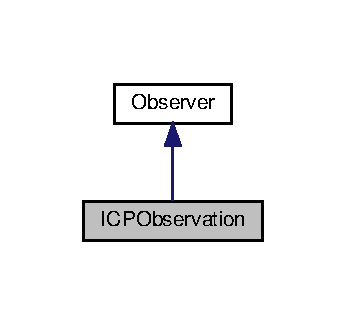
\includegraphics[width=166pt]{classICPObservation__inherit__graph}
\end{center}
\end{figure}


Collaboration diagram for I\+C\+P\+Observation\+:
\nopagebreak
\begin{figure}[H]
\begin{center}
\leavevmode
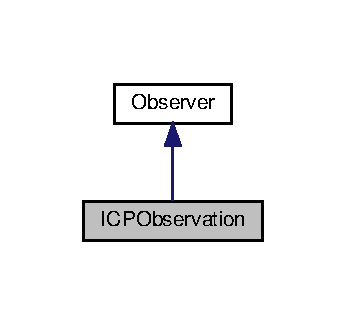
\includegraphics[width=166pt]{classICPObservation__coll__graph}
\end{center}
\end{figure}
\subsection*{Public Member Functions}
\begin{DoxyCompactItemize}
\item 
\mbox{\Hypertarget{classICPObservation_ab062de662cf7f05f9c29d99498bf4e88}\label{classICPObservation_ab062de662cf7f05f9c29d99498bf4e88}} 
void {\bfseries receive\+\_\+message} (const nav\+\_\+msgs\+::\+Odometry\+::\+Const\+Ptr \&msg)
\end{DoxyCompactItemize}
\subsection*{Additional Inherited Members}


The documentation for this class was generated from the following file\+:\begin{DoxyCompactItemize}
\item 
/home/stew/src/catkin/src/localiser/include/localiser/observer.\+hpp\end{DoxyCompactItemize}

\hypertarget{classImuMeasurement}{}\section{Imu\+Measurement Class Reference}
\label{classImuMeasurement}\index{Imu\+Measurement@{Imu\+Measurement}}


Inheritance diagram for Imu\+Measurement\+:
\nopagebreak
\begin{figure}[H]
\begin{center}
\leavevmode
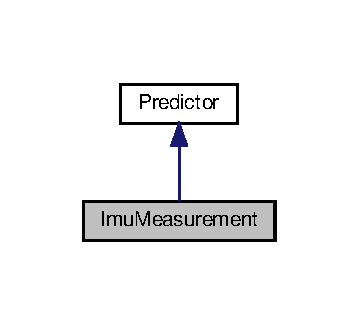
\includegraphics[width=172pt]{classImuMeasurement__inherit__graph}
\end{center}
\end{figure}


Collaboration diagram for Imu\+Measurement\+:
\nopagebreak
\begin{figure}[H]
\begin{center}
\leavevmode
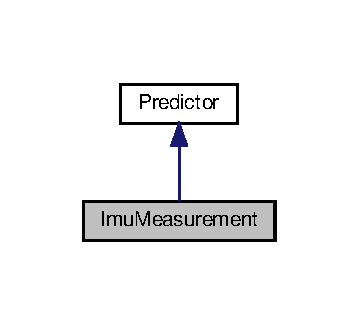
\includegraphics[width=172pt]{classImuMeasurement__coll__graph}
\end{center}
\end{figure}
\subsection*{Public Member Functions}
\begin{DoxyCompactItemize}
\item 
\mbox{\Hypertarget{classImuMeasurement_a66fbe1376e888c8dc7d4062f2ec1dfdd}\label{classImuMeasurement_a66fbe1376e888c8dc7d4062f2ec1dfdd}} 
void {\bfseries receive\+\_\+message} (const sensor\+\_\+msgs\+::\+Imu\+::\+Const\+Ptr \&msg)
\end{DoxyCompactItemize}
\subsection*{Additional Inherited Members}


The documentation for this class was generated from the following file\+:\begin{DoxyCompactItemize}
\item 
/home/stew/src/catkin/src/localiser/include/localiser/predictor.\+hpp\end{DoxyCompactItemize}

\hypertarget{classLocalisationMethod}{}\section{Localisation\+Method Class Reference}
\label{classLocalisationMethod}\index{Localisation\+Method@{Localisation\+Method}}


Inheritance diagram for Localisation\+Method\+:
\nopagebreak
\begin{figure}[H]
\begin{center}
\leavevmode
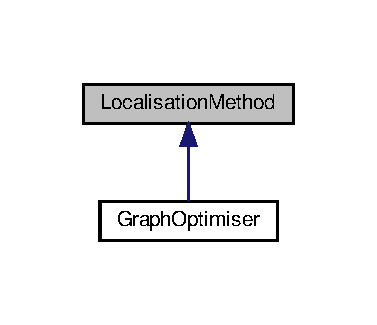
\includegraphics[width=181pt]{classLocalisationMethod__inherit__graph}
\end{center}
\end{figure}
\subsection*{Public Attributes}
\begin{DoxyCompactItemize}
\item 
\mbox{\Hypertarget{classLocalisationMethod_a0a86db738ecb379804ed9d76de46ffb9}\label{classLocalisationMethod_a0a86db738ecb379804ed9d76de46ffb9}} 
std\+::function$<$ void(Eigen\+::\+Vector3d \&, Eigen\+::\+Vector3d \&, ros\+::\+Time)$>$ \hyperlink{classLocalisationMethod_a0a86db738ecb379804ed9d76de46ffb9}{publish\+\_\+odometry}
\begin{DoxyCompactList}\small\item\em Callback to publish odometry information. \end{DoxyCompactList}\item 
\mbox{\Hypertarget{classLocalisationMethod_a51eb7bef9c72bb0cd2e9331ad3080110}\label{classLocalisationMethod_a51eb7bef9c72bb0cd2e9331ad3080110}} 
std\+::function$<$ void(Eigen\+::\+Vector3d \&, Eigen\+::\+Vector3d \&, ros\+::\+Time)$>$ \hyperlink{classLocalisationMethod_a51eb7bef9c72bb0cd2e9331ad3080110}{publish\+\_\+map}
\begin{DoxyCompactList}\small\item\em Callback to publish map information. \end{DoxyCompactList}\item 
\mbox{\Hypertarget{classLocalisationMethod_a18a06e2d38902635f797d09df562d915}\label{classLocalisationMethod_a18a06e2d38902635f797d09df562d915}} 
Eigen\+::\+Vector3d {\bfseries map\+\_\+state}
\item 
\mbox{\Hypertarget{classLocalisationMethod_a0b6e83804c6756388ed8887d1840d67f}\label{classLocalisationMethod_a0b6e83804c6756388ed8887d1840d67f}} 
Eigen\+::\+Vector3d {\bfseries odom\+\_\+state}
\item 
\mbox{\Hypertarget{classLocalisationMethod_aa0b84506c1eb7a791f3700b7c06bc4e2}\label{classLocalisationMethod_aa0b84506c1eb7a791f3700b7c06bc4e2}} 
ros\+::\+Time {\bfseries previous\+\_\+prediction\+\_\+stamp}
\item 
\mbox{\Hypertarget{classLocalisationMethod_a7f89f517fd94361ceb6e42043d788f88}\label{classLocalisationMethod_a7f89f517fd94361ceb6e42043d788f88}} 
ros\+::\+Time {\bfseries previous\+\_\+observation\+\_\+stamp}
\end{DoxyCompactItemize}


The documentation for this class was generated from the following file\+:\begin{DoxyCompactItemize}
\item 
/home/stew/src/catkin/src/localiser/include/localiser/graph\+\_\+optimiser.\+hpp\end{DoxyCompactItemize}

\hypertarget{classLocaliser}{}\section{Localiser Class Reference}
\label{classLocaliser}\index{Localiser@{Localiser}}


The class that manages the localisation process.  




{\ttfamily \#include $<$localiser.\+hpp$>$}

\subsection*{Public Member Functions}
\begin{DoxyCompactItemize}
\item 
\mbox{\Hypertarget{classLocaliser_a1e72dc8f361cd5f00da091b643e9559f}\label{classLocaliser_a1e72dc8f361cd5f00da091b643e9559f}} 
void {\bfseries Set\+Pitch} (double pitch, double variance, ros\+::\+Time stamp)
\item 
\mbox{\Hypertarget{classLocaliser_afa9a61082990c70753d1f9f99e2cd399}\label{classLocaliser_afa9a61082990c70753d1f9f99e2cd399}} 
void {\bfseries Set\+Speed} (double speed, double variance, ros\+::\+Time stamp)
\item 
\mbox{\Hypertarget{classLocaliser_a59f0010ddd53fda3de767b5b7326e216}\label{classLocaliser_a59f0010ddd53fda3de767b5b7326e216}} 
void {\bfseries Set\+Yaw\+Rate} (double yaw\+\_\+rate, double variance, ros\+::\+Time stamp)
\item 
void \hyperlink{classLocaliser_abade968177dc4e68313125ef2bd57756}{Predict} (ros\+::\+Time stamp)
\begin{DoxyCompactList}\small\item\em Perform a prediction update step. \end{DoxyCompactList}\item 
\mbox{\Hypertarget{classLocaliser_a7907cc8b36f2495f3cb6cde2f3bc3ab1}\label{classLocaliser_a7907cc8b36f2495f3cb6cde2f3bc3ab1}} 
void \hyperlink{classLocaliser_a7907cc8b36f2495f3cb6cde2f3bc3ab1}{Update} (Eigen\+::\+Vector3d \&observation, Eigen\+::\+Vector3d \&covariance, ros\+::\+Time stamp)
\begin{DoxyCompactList}\small\item\em Perform the update. \end{DoxyCompactList}\end{DoxyCompactItemize}
\subsection*{Public Attributes}
\begin{DoxyCompactItemize}
\item 
\mbox{\Hypertarget{classLocaliser_af141bf48f966e07742ce51ebb2342544}\label{classLocaliser_af141bf48f966e07742ce51ebb2342544}} 
std\+::function$<$ void(Eigen\+::\+Vector3d \&, Eigen\+::\+Vector3d \&, ros\+::\+Time)$>$ \hyperlink{classLocaliser_af141bf48f966e07742ce51ebb2342544}{perform\+\_\+update}
\begin{DoxyCompactList}\small\item\em Pass the update vector to the localisation method. \end{DoxyCompactList}\item 
\mbox{\Hypertarget{classLocaliser_a2a03c3f46992c40b22e96651fa431e3b}\label{classLocaliser_a2a03c3f46992c40b22e96651fa431e3b}} 
std\+::function$<$ void(Eigen\+::\+Vector2d \&, Eigen\+::\+Vector2d \&, ros\+::\+Time)$>$ \hyperlink{classLocaliser_a2a03c3f46992c40b22e96651fa431e3b}{perform\+\_\+prediction}
\begin{DoxyCompactList}\small\item\em Pass the prediction vector to the localisation method. \end{DoxyCompactList}\item 
\mbox{\Hypertarget{classLocaliser_ad4afb745feaf02272efa67b5d99dface}\label{classLocaliser_ad4afb745feaf02272efa67b5d99dface}} 
std\+::vector$<$ std\+::shared\+\_\+ptr$<$ \hyperlink{classPredictor}{Predictor} $>$ $>$ {\bfseries predictors}
\item 
\mbox{\Hypertarget{classLocaliser_a7eadebb6cc19d5fa8277c8edf90cc325}\label{classLocaliser_a7eadebb6cc19d5fa8277c8edf90cc325}} 
std\+::vector$<$ std\+::shared\+\_\+ptr$<$ \hyperlink{classObserver}{Observer} $>$ $>$ {\bfseries observers}
\end{DoxyCompactItemize}


\subsection{Detailed Description}
The class that manages the localisation process. 

\subsection{Member Function Documentation}
\mbox{\Hypertarget{classLocaliser_abade968177dc4e68313125ef2bd57756}\label{classLocaliser_abade968177dc4e68313125ef2bd57756}} 
\index{Localiser@{Localiser}!Predict@{Predict}}
\index{Predict@{Predict}!Localiser@{Localiser}}
\subsubsection{\texorpdfstring{Predict()}{Predict()}}
{\footnotesize\ttfamily void Localiser\+::\+Predict (\begin{DoxyParamCaption}\item[{ros\+::\+Time}]{stamp }\end{DoxyParamCaption})}



Perform a prediction update step. 

The 2d component (horizontal) of the robot speed. 

The documentation for this class was generated from the following files\+:\begin{DoxyCompactItemize}
\item 
/home/stew/src/catkin/src/localiser/include/localiser/localiser.\+hpp\item 
/home/stew/src/catkin/src/localiser/src/localiser.\+cpp\end{DoxyCompactItemize}

\hypertarget{classObserver}{}\section{Observer Class Reference}
\label{classObserver}\index{Observer@{Observer}}


The base class for providing observations Class type that gives an observation of the current robot pose in the global frame of reference.  




{\ttfamily \#include $<$observer.\+hpp$>$}



Inheritance diagram for Observer\+:
\nopagebreak
\begin{figure}[H]
\begin{center}
\leavevmode
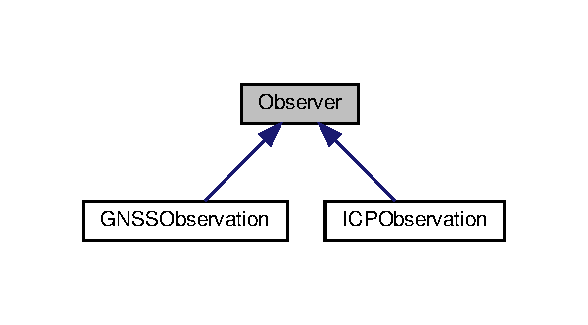
\includegraphics[width=282pt]{classObserver__inherit__graph}
\end{center}
\end{figure}
\subsection*{Public Attributes}
\begin{DoxyCompactItemize}
\item 
\mbox{\Hypertarget{classObserver_acfc1e4a0a7bbd59ccd2da9fda03a2c7e}\label{classObserver_acfc1e4a0a7bbd59ccd2da9fda03a2c7e}} 
std\+::function$<$ void(Eigen\+::\+Vector3d \&, Eigen\+::\+Vector3d \&, ros\+::\+Time)$>$ \hyperlink{classObserver_acfc1e4a0a7bbd59ccd2da9fda03a2c7e}{perform\+\_\+update}
\begin{DoxyCompactList}\small\item\em Perform the prediction. \end{DoxyCompactList}\end{DoxyCompactItemize}


\subsection{Detailed Description}
The base class for providing observations Class type that gives an observation of the current robot pose in the global frame of reference. 

The documentation for this class was generated from the following files\+:\begin{DoxyCompactItemize}
\item 
/home/stew/src/catkin/src/localiser/include/localiser/observer.\+hpp\item 
/home/stew/src/catkin/src/localiser/src/observer.\+cpp\end{DoxyCompactItemize}

\hypertarget{classPredictor}{}\section{Predictor Class Reference}
\label{classPredictor}\index{Predictor@{Predictor}}


The base class for predictive inputs Class type that gives an informed prediction about the future relative location of the robot (given some relative sensor information)  




{\ttfamily \#include $<$predictor.\+hpp$>$}



Inheritance diagram for Predictor\+:
\nopagebreak
\begin{figure}[H]
\begin{center}
\leavevmode
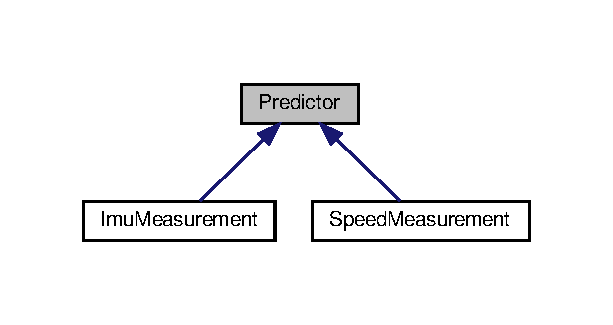
\includegraphics[width=294pt]{classPredictor__inherit__graph}
\end{center}
\end{figure}
\subsection*{Public Attributes}
\begin{DoxyCompactItemize}
\item 
\mbox{\Hypertarget{classPredictor_a068ceee33f66ecad531408cc499efa9d}\label{classPredictor_a068ceee33f66ecad531408cc499efa9d}} 
std\+::function$<$ void(ros\+::\+Time)$>$ \hyperlink{classPredictor_a068ceee33f66ecad531408cc499efa9d}{perform\+\_\+prediction}
\begin{DoxyCompactList}\small\item\em Perform the prediction. \end{DoxyCompactList}\item 
\mbox{\Hypertarget{classPredictor_a30bdde13b4f9510fc93d7ec878d2ccd4}\label{classPredictor_a30bdde13b4f9510fc93d7ec878d2ccd4}} 
std\+::function$<$ void(double, double, ros\+::\+Time)$>$ \hyperlink{classPredictor_a30bdde13b4f9510fc93d7ec878d2ccd4}{update\+\_\+yaw\+\_\+rate}
\begin{DoxyCompactList}\small\item\em Update the yaw rate (and variance) of the robot in radians per second. \end{DoxyCompactList}\item 
\mbox{\Hypertarget{classPredictor_a4cb933efbb1a623cc8983e30cee18e0c}\label{classPredictor_a4cb933efbb1a623cc8983e30cee18e0c}} 
std\+::function$<$ void(double, double, ros\+::\+Time)$>$ \hyperlink{classPredictor_a4cb933efbb1a623cc8983e30cee18e0c}{update\+\_\+speed}
\begin{DoxyCompactList}\small\item\em Update the speed (and variance) of the robot in meters per second. \end{DoxyCompactList}\item 
\mbox{\Hypertarget{classPredictor_a71c837f66a7964d532474020b899c61c}\label{classPredictor_a71c837f66a7964d532474020b899c61c}} 
std\+::function$<$ void(double, double, ros\+::\+Time)$>$ \hyperlink{classPredictor_a71c837f66a7964d532474020b899c61c}{update\+\_\+pitch}
\begin{DoxyCompactList}\small\item\em Update the absolute pitch (and variance) angle of the robot (in radians) \end{DoxyCompactList}\end{DoxyCompactItemize}


\subsection{Detailed Description}
The base class for predictive inputs Class type that gives an informed prediction about the future relative location of the robot (given some relative sensor information) 

The documentation for this class was generated from the following files\+:\begin{DoxyCompactItemize}
\item 
/home/stew/src/catkin/src/localiser/include/localiser/predictor.\+hpp\item 
/home/stew/src/catkin/src/localiser/src/predictor.\+cpp\end{DoxyCompactItemize}

\hypertarget{classROSLocaliser}{}\section{R\+O\+S\+Localiser Class Reference}
\label{classROSLocaliser}\index{R\+O\+S\+Localiser@{R\+O\+S\+Localiser}}


The class that manages the localisation process.  




{\ttfamily \#include $<$ros\+\_\+localiser.\+hpp$>$}

\subsection*{Public Member Functions}
\begin{DoxyCompactItemize}
\item 
\mbox{\Hypertarget{classROSLocaliser_a87eb20c0496eb78fbf79b02047b0583d}\label{classROSLocaliser_a87eb20c0496eb78fbf79b02047b0583d}} 
void {\bfseries Initialise} ()
\item 
\mbox{\Hypertarget{classROSLocaliser_a3b64a321509d2c85146ea469d544f8c8}\label{classROSLocaliser_a3b64a321509d2c85146ea469d544f8c8}} 
void \hyperlink{classROSLocaliser_a3b64a321509d2c85146ea469d544f8c8}{Publish\+Odometry} (Eigen\+::\+Vector3d \&odometry, Eigen\+::\+Vector3d \&covariance, ros\+::\+Time stamp)
\begin{DoxyCompactList}\small\item\em Perform the prediction. \end{DoxyCompactList}\end{DoxyCompactItemize}
\subsection*{Public Attributes}
\begin{DoxyCompactItemize}
\item 
\mbox{\Hypertarget{classROSLocaliser_abe99883c01170dfcc60a88b88328ae32}\label{classROSLocaliser_abe99883c01170dfcc60a88b88328ae32}} 
std\+::shared\+\_\+ptr$<$ \hyperlink{classLocaliser}{Localiser} $>$ {\bfseries localiser}
\item 
\mbox{\Hypertarget{classROSLocaliser_a44b1094cd2f22b428c749a40ba1448cc}\label{classROSLocaliser_a44b1094cd2f22b428c749a40ba1448cc}} 
std\+::vector$<$ ros\+::\+Subscriber $>$ {\bfseries subscribers}
\item 
\mbox{\Hypertarget{classROSLocaliser_a58e3e5be6d6fc11358d603891592c49e}\label{classROSLocaliser_a58e3e5be6d6fc11358d603891592c49e}} 
std\+::shared\+\_\+ptr$<$ \hyperlink{classImuMeasurement}{Imu\+Measurement} $>$ {\bfseries imu}
\item 
\mbox{\Hypertarget{classROSLocaliser_a3fc7a190f5a5d5655a28c2b4b4f1289f}\label{classROSLocaliser_a3fc7a190f5a5d5655a28c2b4b4f1289f}} 
std\+::shared\+\_\+ptr$<$ \hyperlink{classSpeedMeasurement}{Speed\+Measurement} $>$ {\bfseries speed}
\item 
\mbox{\Hypertarget{classROSLocaliser_ac03dc811fd3ab83a58b1d0b4622aae59}\label{classROSLocaliser_ac03dc811fd3ab83a58b1d0b4622aae59}} 
std\+::shared\+\_\+ptr$<$ \hyperlink{classICPObservation}{I\+C\+P\+Observation} $>$ {\bfseries map\+\_\+icp}
\item 
\mbox{\Hypertarget{classROSLocaliser_a3d8f0d6a48173cbde2bb7197992cf720}\label{classROSLocaliser_a3d8f0d6a48173cbde2bb7197992cf720}} 
std\+::shared\+\_\+ptr$<$ \hyperlink{classGNSSObservation}{G\+N\+S\+S\+Observation} $>$ {\bfseries gnss}
\item 
\mbox{\Hypertarget{classROSLocaliser_ab4def0822d196c1693033bac76c834b7}\label{classROSLocaliser_ab4def0822d196c1693033bac76c834b7}} 
std\+::shared\+\_\+ptr$<$ \hyperlink{classGraphOptimiser}{Graph\+Optimiser} $>$ {\bfseries graph\+\_\+optimiser}
\end{DoxyCompactItemize}


\subsection{Detailed Description}
The class that manages the localisation process. 

The documentation for this class was generated from the following files\+:\begin{DoxyCompactItemize}
\item 
/home/stew/src/catkin/src/localiser/include/localiser/ros\+\_\+localiser.\+hpp\item 
/home/stew/src/catkin/src/localiser/src/ros\+\_\+localiser.\+cpp\end{DoxyCompactItemize}

\hypertarget{classSimple__graph}{}\section{Simple\+\_\+graph Class Reference}
\label{classSimple__graph}\index{Simple\+\_\+graph@{Simple\+\_\+graph}}
\subsection*{Public Member Functions}
\begin{DoxyCompactItemize}
\item 
\mbox{\Hypertarget{classSimple__graph_a62344f211bd74de6ff43d9a58f0dd60c}\label{classSimple__graph_a62344f211bd74de6ff43d9a58f0dd60c}} 
{\bfseries Simple\+\_\+graph} (float gps\+\_\+interval, Sparse\+Optimizer $\ast$global\+\_\+optimizer\+\_\+ptr)
\item 
\mbox{\Hypertarget{classSimple__graph_ae152a92b73c6a25c23d43e3e883806ec}\label{classSimple__graph_ae152a92b73c6a25c23d43e3e883806ec}} 
\hyperlink{structSimple__node}{Simple\+\_\+node} $\ast$ {\bfseries propose\+\_\+new\+\_\+node} (double easting, double northing, \hyperlink{structSimple__node}{Simple\+\_\+node} $\ast$current\+\_\+node, unsigned int robot\+\_\+pose\+\_\+id, bool \&added\+\_\+new\+\_\+node)
\item 
\mbox{\Hypertarget{classSimple__graph_aa0f34774a8e313ab1f8cf15a6e8bd2be}\label{classSimple__graph_aa0f34774a8e313ab1f8cf15a6e8bd2be}} 
\hyperlink{structSimple__node}{Simple\+\_\+node} $\ast$ {\bfseries insert\+Node} (double easting, double northing, unsigned int robot\+\_\+pose\+\_\+id)
\item 
\mbox{\Hypertarget{classSimple__graph_ad056ec6e053c97da0d476181a51dfaaf}\label{classSimple__graph_ad056ec6e053c97da0d476181a51dfaaf}} 
void {\bfseries insert\+Edge} (unsigned int node\+\_\+id\+\_\+1, unsigned int node\+\_\+id\+\_\+2)
\item 
\mbox{\Hypertarget{classSimple__graph_a20b92b58d524ee4c1dd4a8cb02378e3a}\label{classSimple__graph_a20b92b58d524ee4c1dd4a8cb02378e3a}} 
unsigned int {\bfseries size} ()
\item 
\mbox{\Hypertarget{classSimple__graph_a7aad6c39497e7e5afde5a5e55a518c8a}\label{classSimple__graph_a7aad6c39497e7e5afde5a5e55a518c8a}} 
void {\bfseries B\+F\+S\+Load\+Simplemap} (mrpt\+::maps\+::\+C\+Simple\+Points\+Map \&landmark\+\_\+map, unsigned int query\+\_\+node\+\_\+id, int terminate\+\_\+depth, std\+::map$<$ unsigned int, std\+::pair$<$ unsigned int, unsigned int $>$$>$ \&corresponding\+\_\+id)
\end{DoxyCompactItemize}


The documentation for this class was generated from the following files\+:\begin{DoxyCompactItemize}
\item 
/home/stew/src/catkin/src/localiser/include/localiser/simple\+\_\+graph.\+h\item 
/home/stew/src/catkin/src/localiser/src/simple\+\_\+graph.\+cpp\end{DoxyCompactItemize}

\hypertarget{structSimple__node}{}\section{Simple\+\_\+node Struct Reference}
\label{structSimple__node}\index{Simple\+\_\+node@{Simple\+\_\+node}}
\subsection*{Public Attributes}
\begin{DoxyCompactItemize}
\item 
\mbox{\Hypertarget{structSimple__node_a4b40187a12d5b9515e7ea46ab67f1386}\label{structSimple__node_a4b40187a12d5b9515e7ea46ab67f1386}} 
std\+::set$<$ unsigned int $>$ {\bfseries landmarks}
\item 
\mbox{\Hypertarget{structSimple__node_aeab16f54e4528a0e655f315b0708d2d7}\label{structSimple__node_aeab16f54e4528a0e655f315b0708d2d7}} 
std\+::set$<$ unsigned int $>$ {\bfseries robot\+\_\+poses}
\item 
\mbox{\Hypertarget{structSimple__node_aca30ab6a39afa18d2d972c266024eed2}\label{structSimple__node_aca30ab6a39afa18d2d972c266024eed2}} 
std\+::set$<$ unsigned int $>$ {\bfseries related\+\_\+nodes}
\item 
\mbox{\Hypertarget{structSimple__node_a1a7a9ba0d40c19fddc20022951b17b84}\label{structSimple__node_a1a7a9ba0d40c19fddc20022951b17b84}} 
unsigned int {\bfseries node\+\_\+id}
\item 
\mbox{\Hypertarget{structSimple__node_a447fecb43f262fdb5a7656e7fea91c30}\label{structSimple__node_a447fecb43f262fdb5a7656e7fea91c30}} 
double {\bfseries easting}
\item 
\mbox{\Hypertarget{structSimple__node_a9a40a987d23afc35df7285ed59baca13}\label{structSimple__node_a9a40a987d23afc35df7285ed59baca13}} 
double {\bfseries northing}
\end{DoxyCompactItemize}


The documentation for this struct was generated from the following file\+:\begin{DoxyCompactItemize}
\item 
/home/stew/src/catkin/src/localiser/include/localiser/simple\+\_\+graph.\+h\end{DoxyCompactItemize}

\hypertarget{classSpeedMeasurement}{}\section{Speed\+Measurement Class Reference}
\label{classSpeedMeasurement}\index{Speed\+Measurement@{Speed\+Measurement}}


Inheritance diagram for Speed\+Measurement\+:
\nopagebreak
\begin{figure}[H]
\begin{center}
\leavevmode
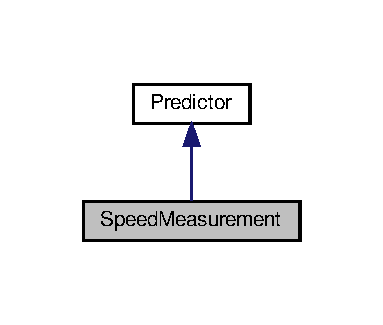
\includegraphics[width=184pt]{classSpeedMeasurement__inherit__graph}
\end{center}
\end{figure}


Collaboration diagram for Speed\+Measurement\+:
\nopagebreak
\begin{figure}[H]
\begin{center}
\leavevmode
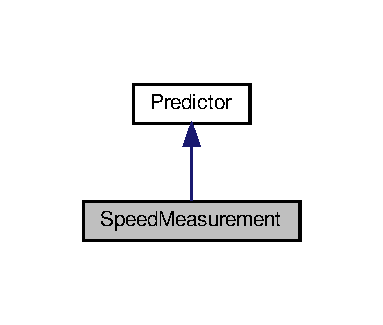
\includegraphics[width=184pt]{classSpeedMeasurement__coll__graph}
\end{center}
\end{figure}
\subsection*{Public Member Functions}
\begin{DoxyCompactItemize}
\item 
\mbox{\Hypertarget{classSpeedMeasurement_adb209fa0d3651ff9e021476367322bc7}\label{classSpeedMeasurement_adb209fa0d3651ff9e021476367322bc7}} 
void {\bfseries receive\+\_\+message} (const nav\+\_\+msgs\+::\+Odometry\+::\+Const\+Ptr \&msg)
\end{DoxyCompactItemize}
\subsection*{Additional Inherited Members}


The documentation for this class was generated from the following file\+:\begin{DoxyCompactItemize}
\item 
/home/stew/src/catkin/src/localiser/include/localiser/predictor.\+hpp\end{DoxyCompactItemize}

%--- End generated contents ---

% Index
\backmatter
\newpage
\phantomsection
\clearemptydoublepage
\addcontentsline{toc}{chapter}{Index}
\printindex

\end{document}
